\documentclass[12pt]{article}
\usepackage{geometry}                % See geometry.pdf to learn the layout options. There are lots.
\geometry{letterpaper}                   % ... or a4paper or a5paper or ... 
%\geometry{landscape}                % Activate for for rotated page geometry
\usepackage[parfill]{parskip}    % Activate to begin paragraphs with an empty line rather than an indent
\usepackage{daves,fancyhdr,natbib,graphicx,dcolumn,amsmath,lastpage,url}
\usepackage{amsmath,amssymb,epstopdf,longtable}
\usepackage{paralist} 
\DeclareGraphicsRule{.tif}{png}{.png}{`convert #1 `dirname #1`/`basename #1 .tif`.png}
\pagestyle{fancy}
\lhead{CE 3372 -- Water Systems Design}
%\rhead{FALL 2010}
%\rhead{SPRING 2011}
%\rhead{FALL 2011}
%\rhead{SPRING 2012}
%\rhead{FALL 2013}
%\rhead{FALL 2016}
\rhead{FALL 2017}
%\lfoot{EXERCISE 1 -- REVISION 1}
%\lfoot{EXERCISE 1 -- REVISION 2}
%\lfoot{EXERCISE 1 -- REVISION 3}
\lfoot{ES 18}
\cfoot{}
\rfoot{Page \thepage\ of \pageref{LastPage}}
\renewcommand\headrulewidth{0pt}



\begin{document}

\begin{center}
\textbf{MEMORANDUM}
%{\textbf{{ CE 3372 -- Water Systems Design} \\ {Exercise Set 2}}}
\end{center}
\begingroup
\begin{tabular}{p{1in} p{5in}}
\hline
\hline
To: & P. N Guin \\ ~\\
From: & P. Olar Bear \\ ~\\
Date: & 04MAR2024 \\ ~\\
Subject: & CE 3372 -- Water Systems Design, Exercise Set 18. ~\\

\hline
\hline
\end{tabular}
\endgroup


\section*{\small{Purpose}}
The purpose of the exercise is to develop expertise in application of gradually varied flow equation in open channel flow, and practice Excel skills for simple geometries.  The exercise is repeated in SWMM in the next exercise.

\section*{\small{Discussion}}
The solution is presented below after re-statement of the problem.  Relevant discussion components are imbedded within the solution.
%%~ & ~ \\
%%ABET General Criteria 3: & (a) \dots apply knowledge of mathematics, science, and engineering  \\
%%~ & (e)  \dots solve engineering problems  \\
%%~ & (k) \dots an ability to use the techniques, skills, and modern engineering tools necessary for engineering practice. \\
%%%~ & ~ \\
%%%Grading Criteria:  & Completion; Correct Solutions; Calculation Details \\
%\end{tabular}
%\endgroup
\section*{\small{Problem Statement}}
\begin{enumerate}
%%%%%%%%%%%%%%%%%%
\item Water flows at a steady rate of 192$ft^3/s$ through a concrete-lined rectangular channel 16 ft wide as depicted in Figure \ref{fig:channel_profile}. The water enters the $0.35 \%$ sloped channel ($S_0 = 0.0035$) at location $1$ and is flowing at $110\%$ normal depth ($1.1 \times y_n$).  The water exits over a 3-foot tall weir (assume sharp-crest weir) at location $2$.\footnote{The water-surface-profile spreadsheet on the class server can be adapted to this problem, or you can create your own.}

\begin{figure}[htbp] %  figure placement: here, top, bottom, or page
   \centering
   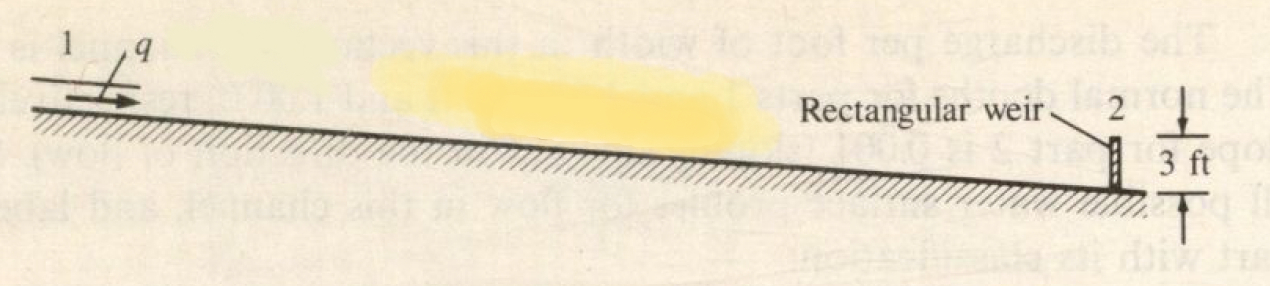
\includegraphics[width=6in]{channel_profile.jpg} 
   \caption{Profile of concrete-lined rectangular channel.}
   \label{fig:channel_profile}
\end{figure}

Determine: 
\begin{enumerate}[i]
\item The critical depth for the channel (in feet).
\item Assuming flow over the weir must pass through critical depth, what is the pool depth just upstream of the weir? (Hint: Add the critical depth to the weir height as an approximation to the pool depth)
\item Using the variable-step method, determine the water-surface profile from location $1$ to location $2$.
\item How far upstream from the weir is the flow at $110\%$ normal depth? (i.e. how far upstream is location $1$ from location $2$.
\item What is the average $\Delta x$ in your computations if the $\Delta y$ is $0.1$ feet?
\item Include sample calculations (if you use a spreadsheet, screen capture a portion of the calculations section).
\item Include a plot of the water surface elevation, and the channel bottom elevation (a profile plot -- like the figure, but with the horizontal distance as the x-axis).
\end{enumerate}

\section*{\small{Solution}}
To address the specific questions the following steps are required:
\begin{enumerate}
\item Build a tool to take Q, n, Width as input. Figure \ref{fig:GVF-UpperLeft} is such a tool with these inputs along the left side of the spreadsheet.
\item Compute normal and critical depth for the channel.
Normal depth is computed using Manning's equation for a rectangular channel, then apply goal seek until the computed flow rate agrees with the prescribed flow rate.  For the supplied problem values the normal depth is about 1.509 feet.  Critical depth is computed settinf the Froude number for the rectangular channel to unity (one) and solving for the required flow depth.  For the supplied problem values the critical depth is about 1.648 feet.
\item Assume depth at weir is weir height+critical depth -- use that as starting value for the numerical method.  For the supplied problem values, the pool depth just upstream of the weir is about 4.648 feet.
\item Use variable step method as outlined in class an compute spacing as depth is changed.  For the supplied values, we start at the weir and compute upstream, using depth increments of 0.1 feet until the depth is at 110\% of normal depth, which for this problem is about 1.66 feet.
%\item If there is a sign change, then there is a hydraulic jump.  Continue after the jump, but remember to reverse the spacings for the plots.
\item Plot the results.
\end{enumerate}

Implementing these steps is shown in Figure \ref{fig:GVF-UpperLeft} and Figure \ref{fig:GVF-LowerLeft}.   Figure \ref{fig:GVF-LowerLeft} is the graphics portion of the spreadsheet that displays the plot.

\begin{figure}[htbp] %  figure placement: here, top, bottom, or page
   \centering
   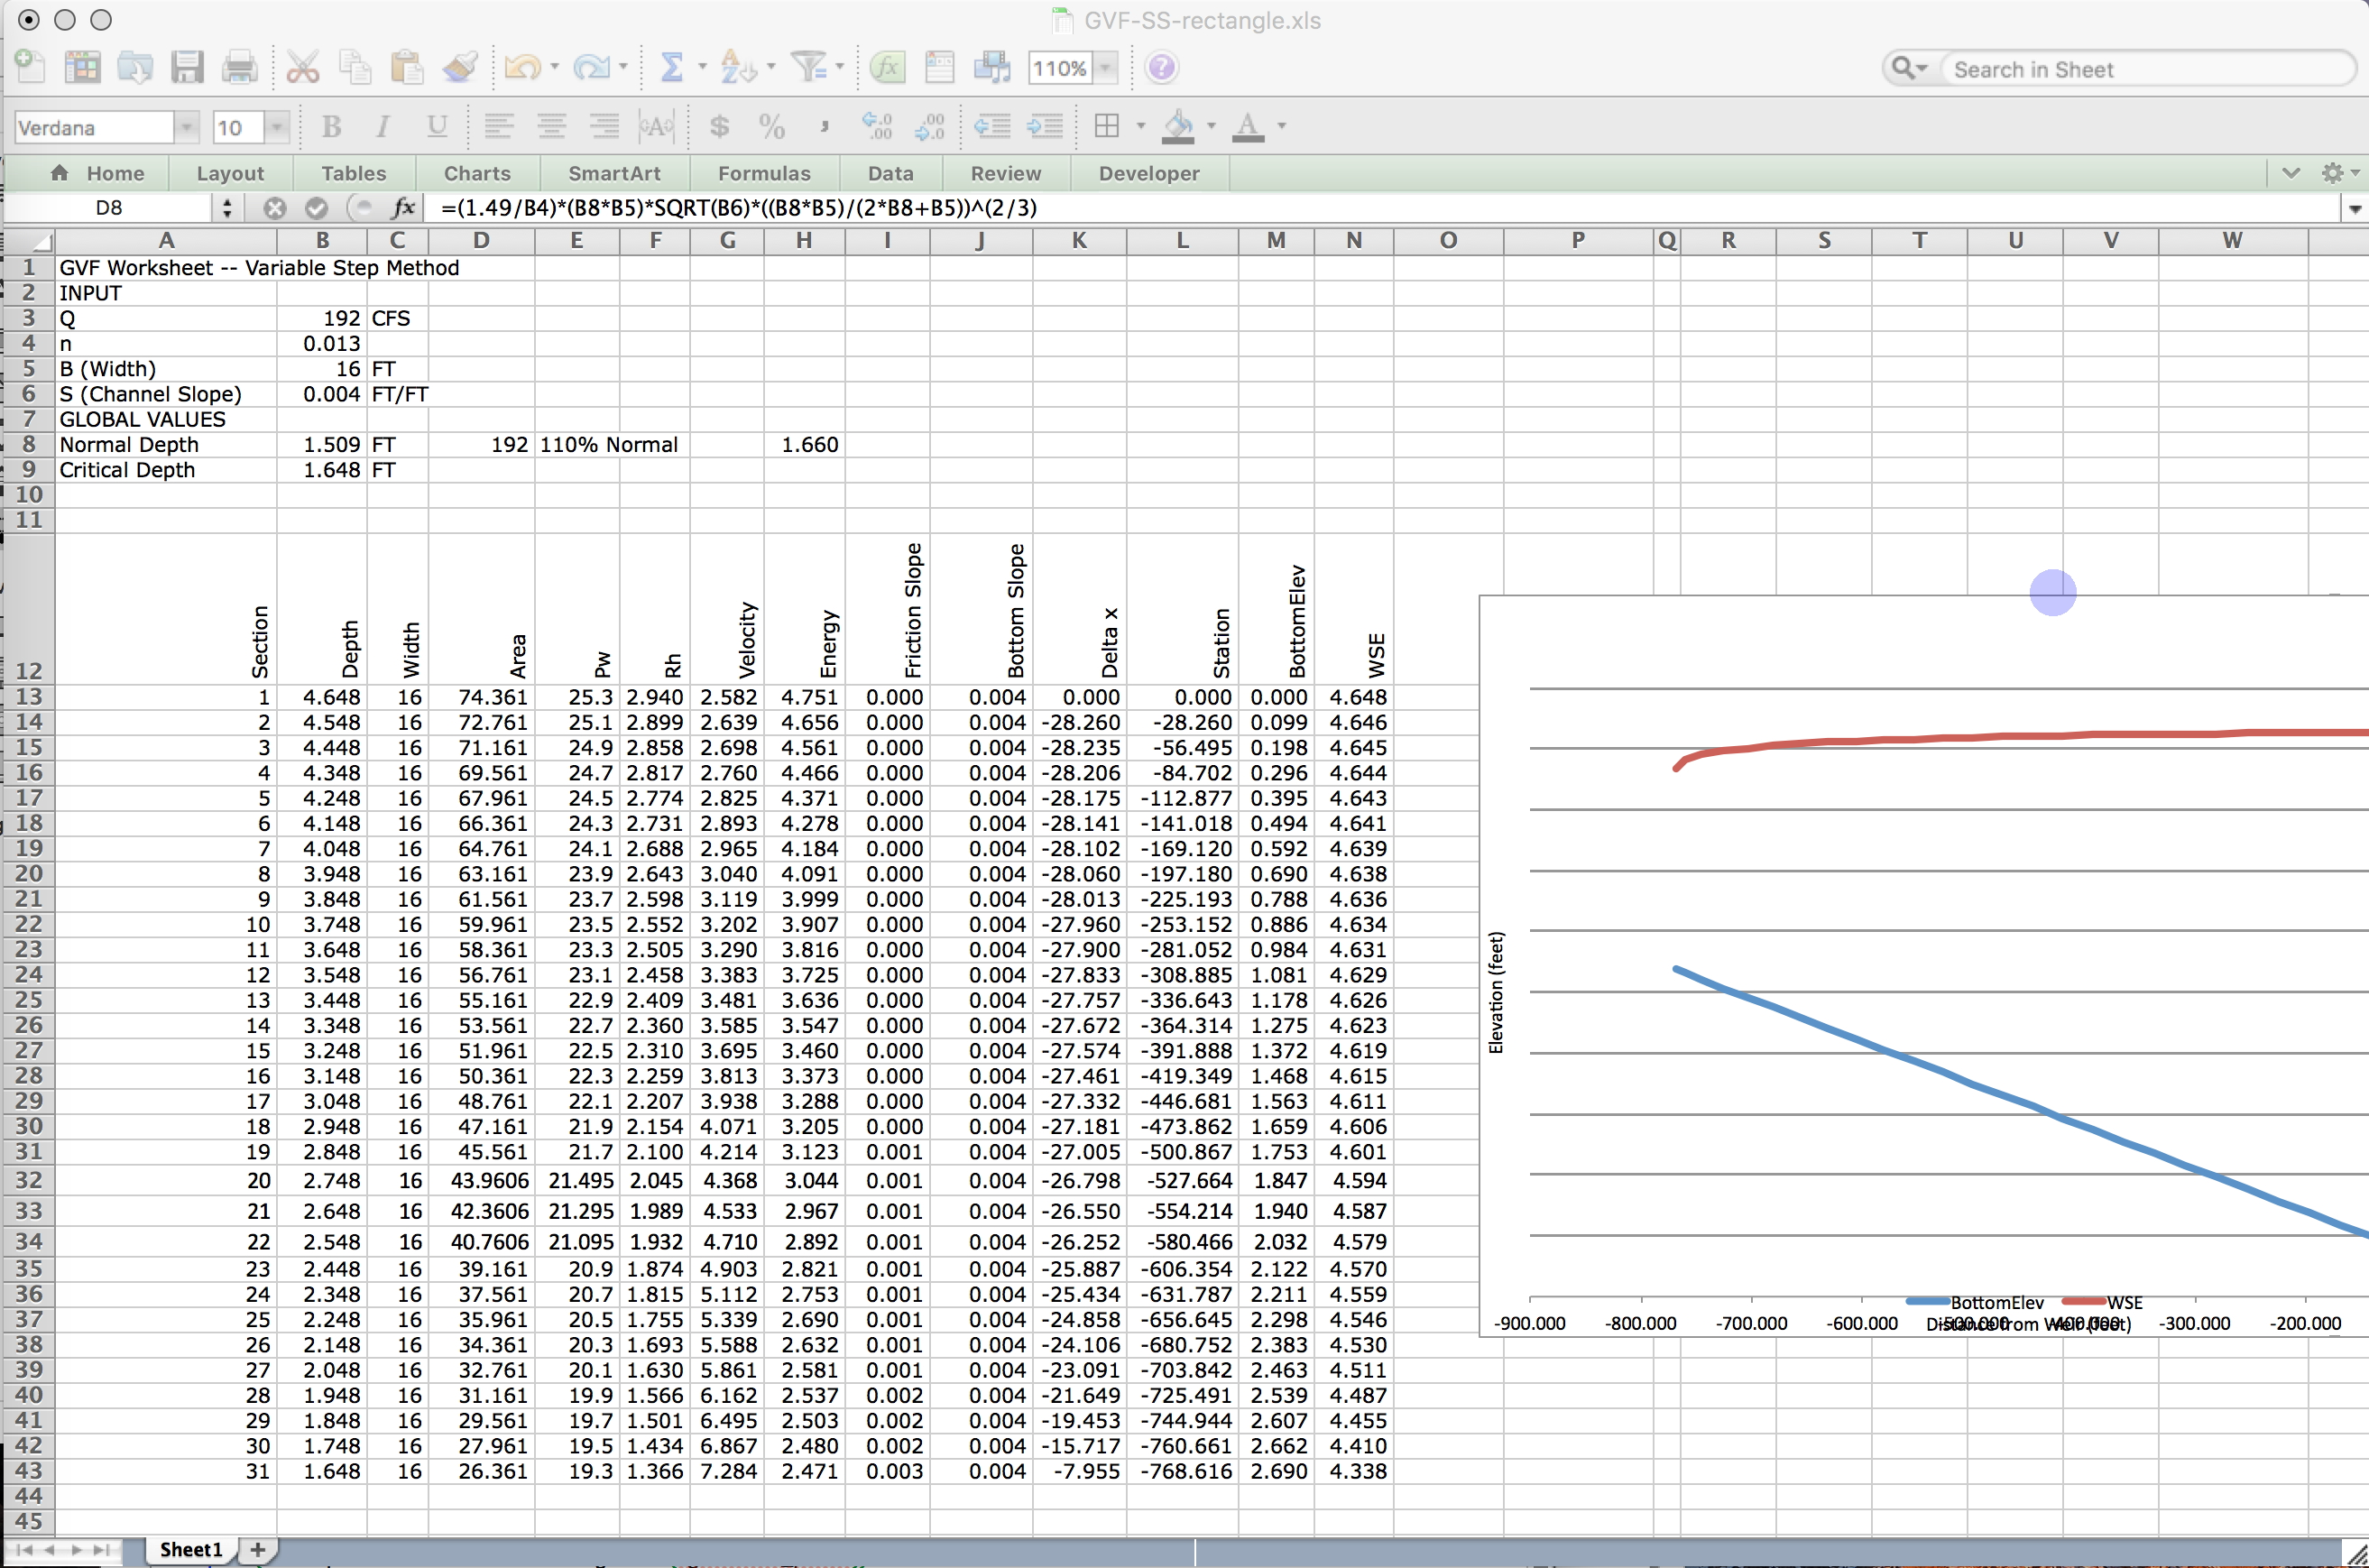
\includegraphics[width=6in]{GVF-UpperLeft.jpg} 
   \caption{GVF Spreadsheet for channel in Figure\ref{fig:channel_profile}}
   \label{fig:GVF-UpperLeft}
\end{figure}
\clearpage

\begin{figure}[htbp] %  figure placement: here, top, bottom, or page
   \centering
   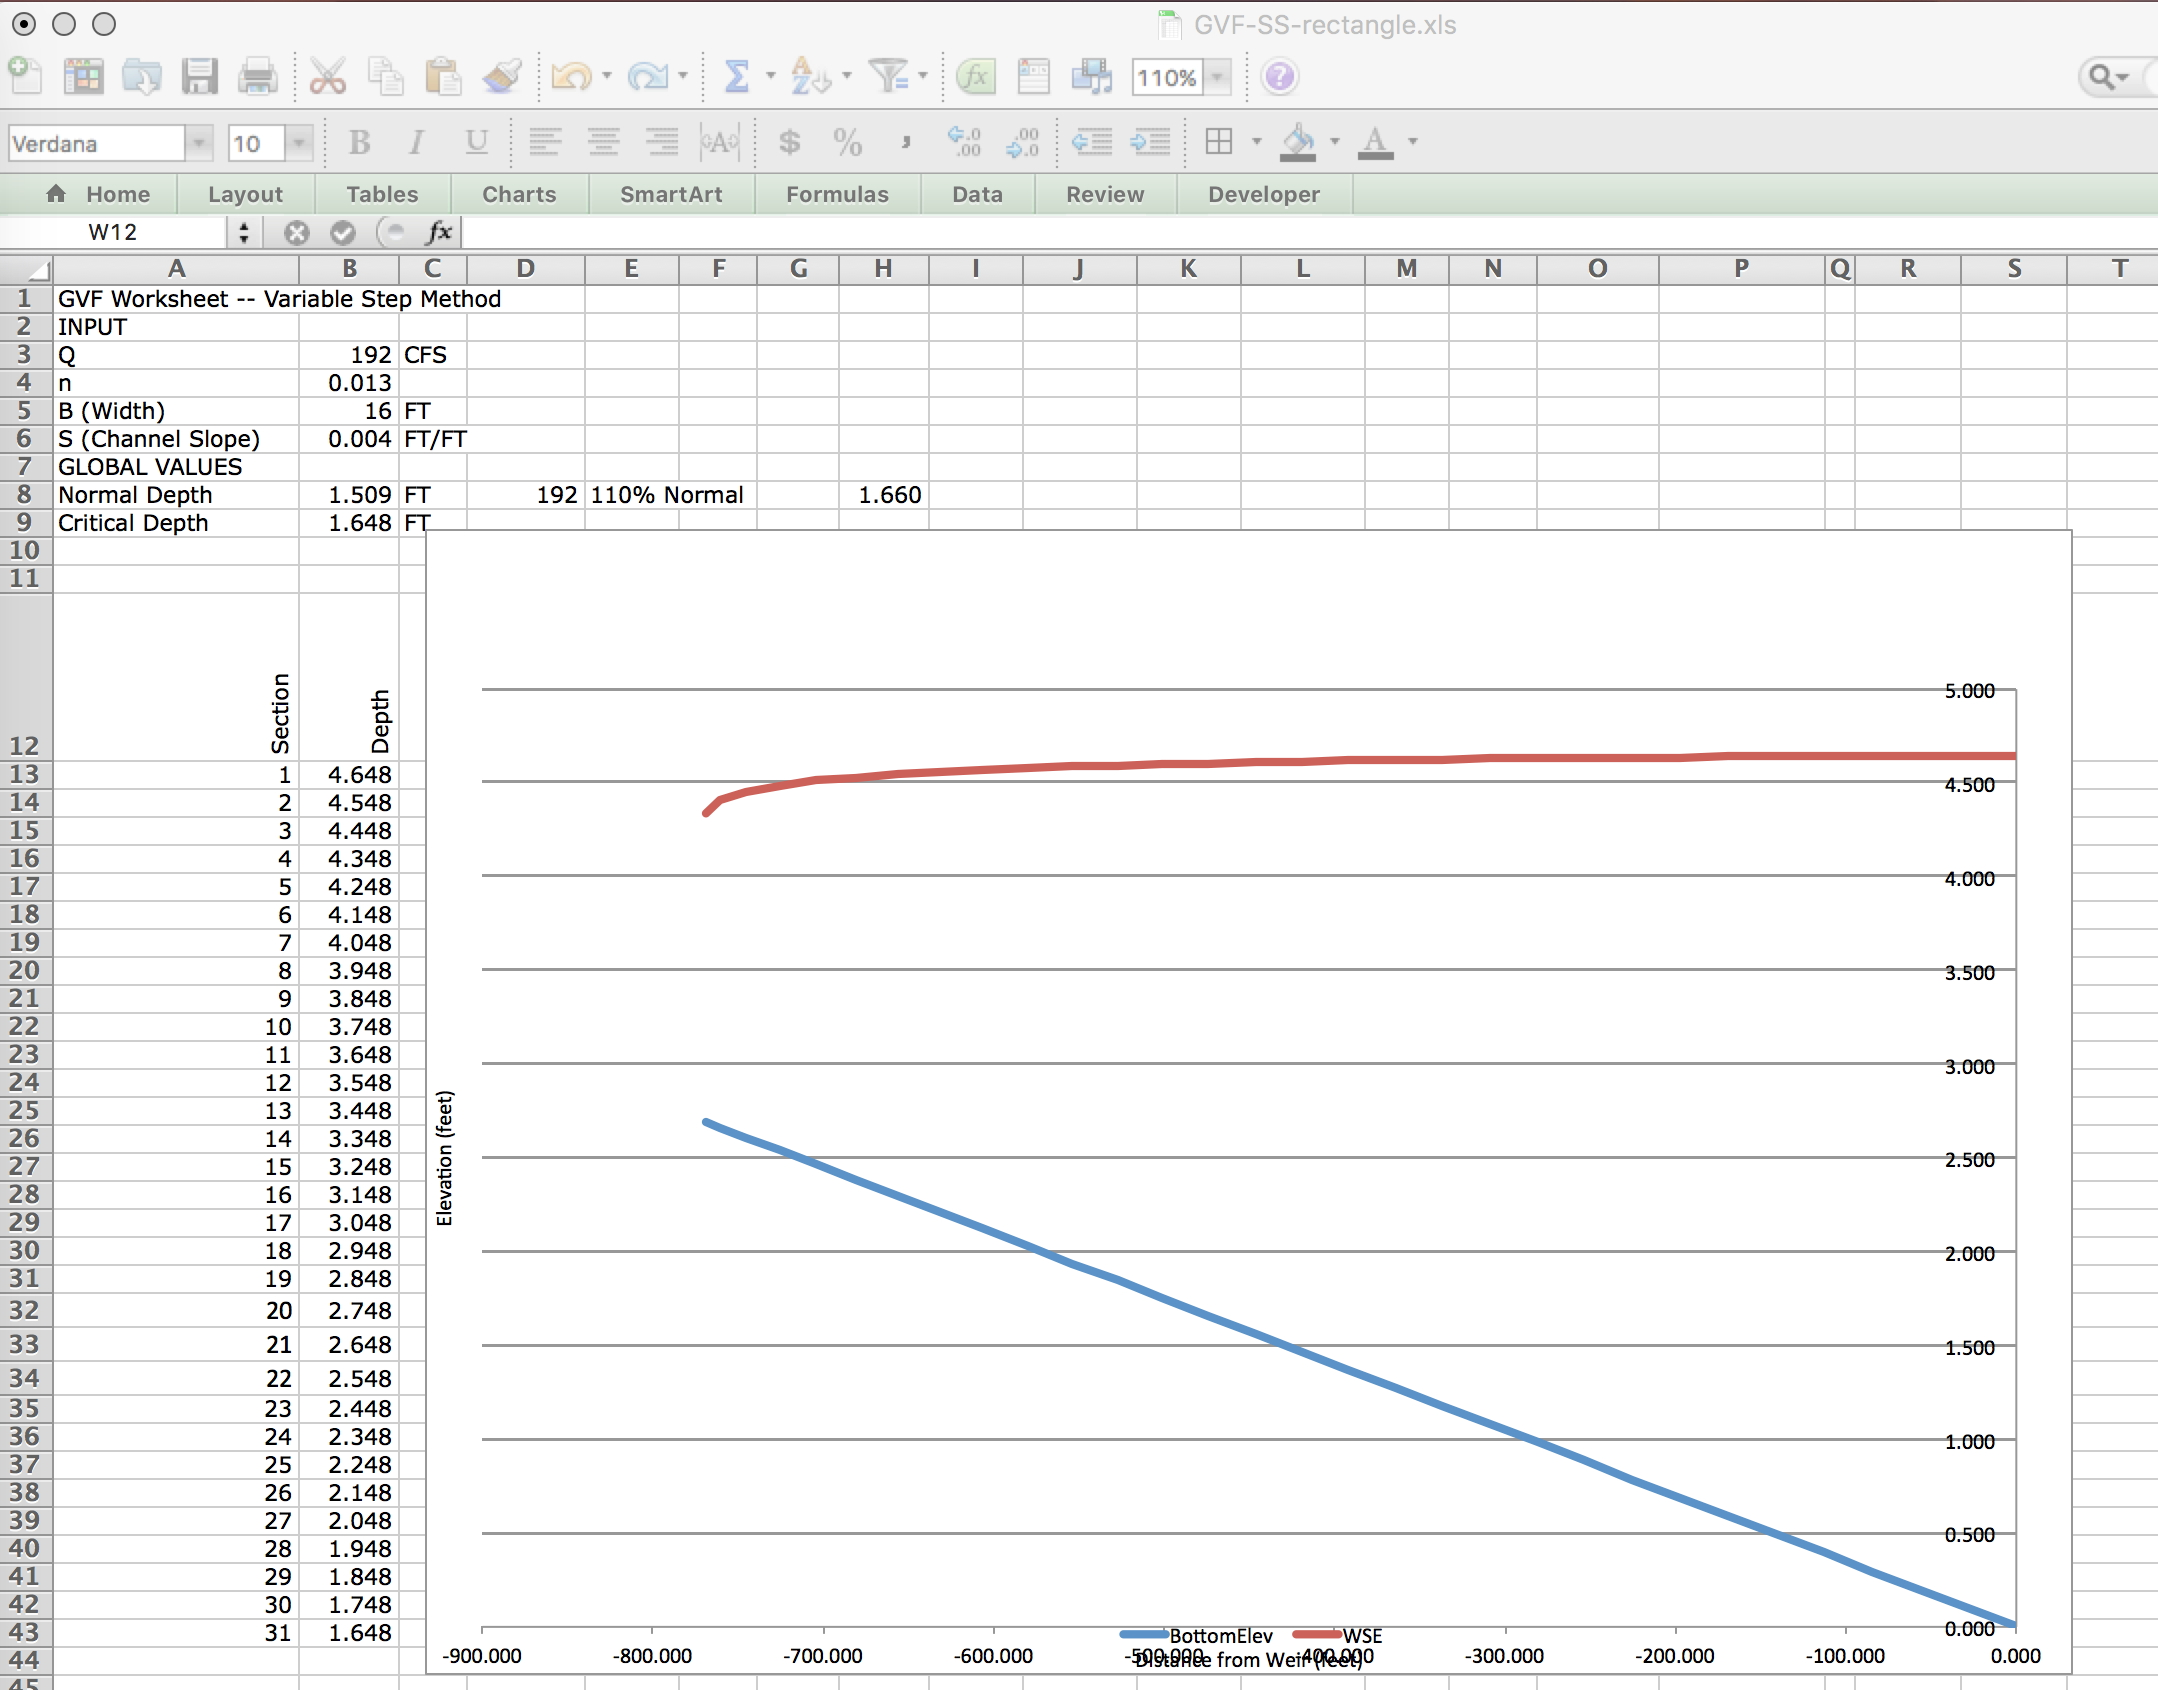
\includegraphics[width=6in]{GVF-LowerLeft.jpg} 
   \caption{GVF Spreadsheet for channel in Figure\ref{fig:channel_profile}}
   \label{fig:GVF-LowerLeft}
\end{figure}


%Figure \ref{fig:GVF-WSPNumbers} are the numerical values that will be used for plotting.  Notice that the stationing still decreases after the jump.  Using the energy equation to locate the jump is just approximate, because energy is lost in the jump, so the WSP upstream of the jump is probably lower than if calculated using a proper momentum balance, but it will be adequately close for this example.    
%
%\begin{figure}[htbp] %  figure placement: here, top, bottom, or page
%   \centering
%   \includegraphics[width=6in]{GVF-WSPNumbers.jpg} 
%   \caption{Approximate flow depth, station, and WSE values for channel in Figure\ref{fig:channel_profile}}
%   \label{fig:GVF-WSPNumbers}
%\end{figure}
%
%\clearpage
%
%Figure \ref{fig:GVF-WSPPlot} is the plot of the water surface and the bottom elevations.  The ``jump'' is pretty obvious in the plot and the location of the jump would be reasonably close to where it is located in the plots.  Energy is lost in the jump and that fact is not reflected in these calculations.
%
%\begin{figure}[htbp] %  figure placement: here, top, bottom, or page
%   \centering
%   \includegraphics[width=6in]{GVF-WSPPlot.jpg} 
%   \caption{Plot of channel bottom and WSE for channel in Figure\ref{fig:channel_profile}}
%   \label{fig:GVF-WSPPlot}
%\end{figure}

The average spacing can be estimated as the total distance $\approx 768 ft.$ divided by the number of reaches (in this solution 30), which is $\approx 25.6 ft.$.   Use this value in the next exercise where the same problem is examined using SWMM. 

%
%\item Repeat the problem, except model the situation in SWMM.
%\begin{enumerate}[i]
%\item Make your SWMM model have conduits that are the average $\Delta x$ from the problem above.
%\item Include a screen capture of your SWMM model showing the computed water-surface-profile.   
%\end{enumerate}
%\clearpage
%\item Estimate the peak flow of a square shaped 50 acre, single family residential area in Harris County. 
%The site is graded from an elevation of 150ft at the corner to 139ft at the outlet as depicted on Figure \ref{fig:watershed.jpg}.
%
%\begin{figure}[h!] %  figure placement: here, top, bottom, or page
%   \centering
%   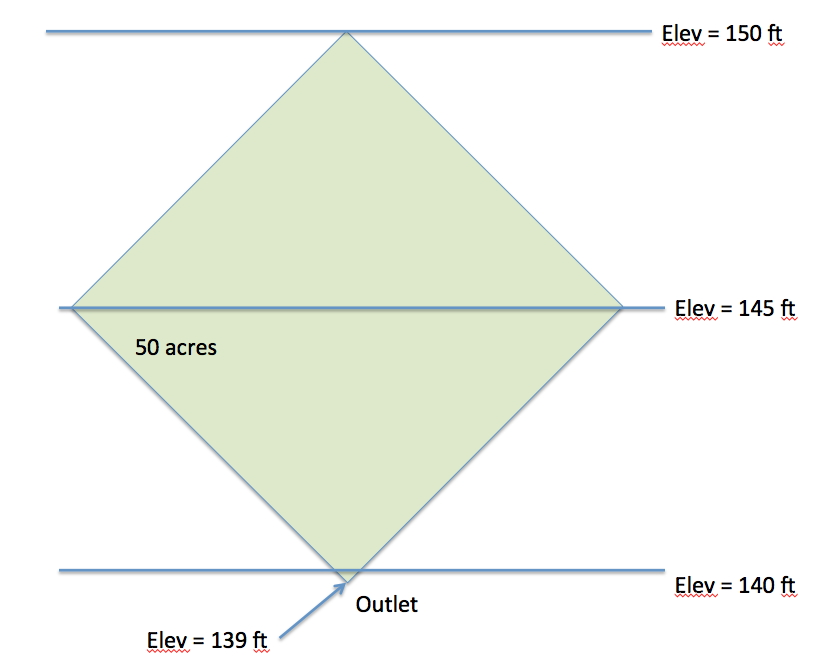
\includegraphics[width=4in]{watershed.jpg} 
%   \caption{50 acre square watershed with elevation contour overlay}
%   \label{fig:watershed.jpg}
%\end{figure} 
%
%\begin{enumerate}[i)]
%\item Draw on the diagram the longest flow path from the highest elevation to the outlet, and determine the length of the flow path in feet.
%\item Estimate the time of concentration.
%\item Estimate the peak discharge for a 10-year, 6-hour storm using the Rational Method.
%\item Use SWMM to simulate the runoff hydrograph from the watershed for a 10-year, 6-hour storm using the NRCS 6-hr Rainfall Distribution Curves (in Lecture Notes).  Include a screen capture of the SWMM model.
%\item Include a screen capture of the sub-catchment dialog box where you supply sub-catchment area, and width.   Describe how you selected your width for your model.   
%\item Determine the calculated peak discharge from the SWMM model and compare its value to the value from the Rational Method.
%\end{enumerate}
%
%%\item A grass-lined roadside swale (ditch) is to be built as a trapezoidal channel to carry 20 cubic-feet per second, with a 1 foot freeboard.   If the desired flow depth is 1 foot, and the right of way available to fit the ditch is 12 feet, what is the required side slope and bottom width.   The longitudinal slope is 1\%.
%%\begin{enumerate}[i]
%%\item Sketch the cross section and label the width, depth, and side slope.
%%\item Write the appropriate relationships between velocity, depth, and discharge for the section.
%%\item Compute the required side-slope in the section.
%%\item Compute the mean section velocity in the section.
%%\end{enumerate}

\end{enumerate}
\end{document}  